\documentclass[12pt, leqno]{article}
\usepackage{amsfonts}
\usepackage{amsmath}
\usepackage{amssymb}
\usepackage{fancyhdr}
\usepackage{hyperref}
\usepackage{tikz}
\usepackage{pgfplots}
\usepackage{listings}

\newcommand{\bbR}{\mathbb{R}}
\newcommand{\bbC}{\mathbb{C}}
\newcommand{\calV}{\mathcal{V}}
\newcommand{\calW}{\mathcal{W}}
\newcommand{\ddiag}{\operatorname{diag}}
\newcommand{\fl}{\operatorname{fl}}
\newcommand{\macheps}{\epsilon_{\mathrm{mach}}}
\newcommand{\matlab}{\textsc{Matlab}}

\newcommand{\hdr}[2]{
  \pagestyle{fancy}
  \lhead{Bindel, Spring 2016}
  \rhead{Numerical Analysis (CS 4220)}
  \fancyfoot{}
  \begin{center}
    {\large{\bf Notes for #1}}
  \end{center}
  \lstset{language=matlab,columns=flexible}  
}


\begin{document}
\hdr{2016-02-22}

\section*{Least squares: the big idea}

Least squares problems are a special sort of minimization problem.
Suppose $A \in \bbR^{m \times n}$ where $m > n$.  In general, we
cannot solve the {\em overdetermined} system $Ax = b$; the best we can do is minimize the
{\em residual} $r = b-Ax$.  In the least squares problem, we minimize
the two norm of the residual:
\[
\mbox{Find } x \mbox{ to minimize } \|r\|_2^2 =
\langle r, r \rangle.
\]
This is not the only way to approximately solve the system, but it
is attractive for several reasons:
\begin{enumerate}
\item It's mathematically attractive: the solution of the least
  squares problem is $x = A^\dagger b$ where $A^\dagger$ is the {\em
    Moore-Penrose pseudoinverse} of $A$.
\item There's a nice picture that goes with it --- the least squares
  solution is the projection of $b$ onto the range of $A$, and the
  residual at the least squares solution is orthogonal to the range of
  $A$.
\item It's a mathematically reasonable choice in statistical settings
  when the data vector $b$ is contaminated by Gaussian noise.
\end{enumerate}

\section*{Cricket chirps: an example}

Did you know that you can estimate the temperature by listening to the
rate of chirps?  The data set in Table~\ref{table1}%
\footnote{Data set originally attributed to
  \url{http://mste.illinois.edu}}.  represents measurements of the
number of chirps (over 15 seconds) of a striped ground cricket at
different temperatures measured in degrees Farenheit.  A plot
(Figure~\ref{fig2}) shows that the two are roughly correlated: the
higher the temperature, the faster the crickets chirp.  We can
quantify this by attempting to fit a linear model
\[
  \mbox{temperature} = \alpha \cdot \mbox{chirps} + \mbox{beta} + \epsilon
\]
where $\epsilon$ is an error term.  To solve this problem by linear
regression, we minimize the residual
\[
  r = b-Ax
\]
where
\begin{align*}
  b_{i} &= \mbox{temperature in experiment } i \\
  A_{i1} &= \mbox{chirps in experiment } i \\
  A_{i2} &= 1 \\
  x &= \begin{bmatrix} \alpha \\ \beta \end{bmatrix}
\end{align*}
MATLAB and Octave are capable of solving least squares problems using
the backslash operator; that is, if {\tt chirps} and {\tt temp} are
column vectors in MATLAB, we can solve this regression problem as
\begin{lstlisting}
  A = [chirps, ones(ndata,1)];
  x = A\temp;
\end{lstlisting}
The algorithms underlying that backslash operation will make up
most of the next lecture.

\begin{figure}
  \begin{center}
    \begin{tikzpicture}
      \begin{axis}[xlabel={Chirps},ylabel={Degrees},grid=major]
        \addplot[only marks] table {2016-02-22-cricket.dat};
        \addplot table[x=chirp,y=fit]{2016-02-22-cricket.dat};
      \end{axis}
    \end{tikzpicture}
  \end{center}
  \caption{Cricket chirps vs.~temperature and a model fit via
    linear regression.}
  \label{fig2}
\end{figure}

\begin{table}
  \small
  \begin{tabular}{l|cccccccccccccccccc}
    Chirp &
    20& 16& 20& 18& 17& 16& 15& 17& 15& 16& 15& 17& 16& 17& 14 \\
    Temp &
    89& 72& 93& 84& 81& 75& 70& 82& 69& 83& 80& 83& 81& 84& 76
  \end{tabular}
  \caption{Cricket data: Chirp count over a 15 second period vs.~temperature
    in degrees Farenheit.}
  \label{table1}
\end{table}

In more complex examples, we want to fit a model involving more than
two variables.  This still leads to a linear least squares problem,
but one in which $A$ may have more than one or two columns.  As we
will see later in the semester, we also use linear least squares
problems as a building block for more complex fitting procedures,
including fitting nonlinear models and models with more complicated
objective functions.

\section*{Normal equations}

\begin{figure} 
  \begin{center}
  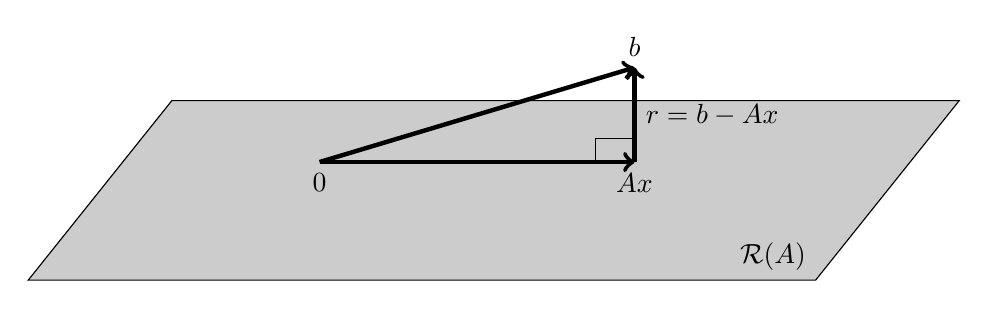
\begin{tikzpicture}
    \begin{scope}[xslant=0.8,xscale=5,yscale=3]
      \draw[fill=black!20] (-0.5,-0.5) rectangle (1.5,0.26);
      \draw[ultra thick,->]
        (0,0) node[below] {$0$} --
        (0.8,0) node[below] {$Ax$};
      \node[above left] at (1.5,-0.5) {$\mathcal{R}(A)$};
    \end{scope}
    \begin{scope}[xscale=5,yscale=3]
    \draw[ultra thick,->]
      (0,0) -- (0.8,0.4) node[above] {$b$};
    \draw[ultra thick,->]
      (0.8,0) -- (0.8,0.4) node[midway,right] {$r=b-Ax$};
    \draw (0.7,0) -- (0.7,0.1) -- (0.8,0.1);
    \end{scope}
  \end{tikzpicture}
  \end{center}
  \caption{Picture of a linear least squares problem.  The vector $Ax$
           is the closest vector in $\mathcal{R}(A)$ to a target
           vector $b$ in the Euclidean norm.  Consequently, the
           residual $r = b-Ax$ is normal (orthogonal) to
           $\mathcal{R}(A)$.}
  \label{fig1}
\end{figure}

When we minimize the Euclidean norm of $r = b-Ax$, we find that $r$ is
{\em normal} to everything in the range space of $A$ (Figure~\ref{fig1}):
\[
  b-Ax \perp \mathcal{R}(A),
\]
or, equivalently, for all $z \in \bbR^n$ we have
\[
  0 = (Az)^T (b-Ax) = z^T(A^T b - A^T A x).
\]
The statement that the residual is orthogonal to everything in
$\mathcal{R}(A)$ thus leads to the {\em normal equations}
\[
  A^T A x = A^T b.
\]
To see why this is the right system, suppose $x$ satisfies the normal
equations and let $y \in \bbR^{n}$ be arbitrary.  Using the fact that
$r \perp Ay$ and the Pythagorean theorem, we have
\[
  \|b-A(x+y)\|^2 = \|r-Ay\|^2 = \|r\|^2 + \|Ay\|^2 > 0.
\]
The inequality is strict if $Ay \neq 0$; and if the columns of
$A$ are linearly independent, $Ay = 0$ is equivalent to $y = 0$.

We can also reach the normal equations by calculus.  Define
the least squares objective function:
\[
  F(x) = \|Ax-b\|^2 = (Ax-b)^T (Ax-b) = x^T A^TA x - 2x^T A^T b + b^T b.
\]
The minimum occurs at a {\em stationary point}; that is,
for any perturbation $\delta x$ to $x$ we have
\[
  \delta F = 2 \delta x^T (A^T A x - A^T b) = 0;
\]
equivalently, $\nabla F(x) = 2 (A^T A x - A^T b) = 0$ ---
the normal equations again!

\section*{A family of factorizations}

\subsection*{Cholesky}

If $A$ is full rank, then $A^T A$ is symmetric and positive definite
matrix, and we can compute a Cholesky factorization of $A^T A$:
\[
  A^T A = R^T R.
\]
The solution to the least squares problem is then
\[
  x = (A^T A)^{-1} A^T b = R^{-1} R^{-T} A^T b,
\]
or, in MATLAB world
\begin{lstlisting}
  R = chol(A'*A, 'upper');
  x = R\(R'\(A'*b));
\end{lstlisting}

\subsection*{Economy QR}

The Cholesky factor $R$ appears in a different setting as well.
Let us write $A = QR$ where $Q = AR^{-1}$; then
\[
  Q^T Q = R^{-T} A^T A R^{-1} = R^{-T} R^T R R^{-1} = I.
\]
That is, $Q$ is a matrix with orthonormal columns.  This
``economy QR factorization'' can be computed in several different
ways, including one that you have seen before in a different guise
(the Gram-Schmidt process).  MATLAB provides a numerically stable
method to compute the QR factorization via
\begin{lstlisting}
  [Q,R] = qr(A,0);
\end{lstlisting}
and we can use the QR factorization directly to solve the least
squares problem without forming $A^T A$ by
\begin{lstlisting}
  [Q,R] = qr(A,0);
  x = R\(Q'*b);
\end{lstlisting}

\subsection*{Full QR}

There is an alternate ``full'' QR decomposition where we write
\[
A = QR, \mbox{ where }
Q = \begin{bmatrix} Q_1 & Q_2 \end{bmatrix} \in \bbR^{n \times n},
R = \begin{bmatrix} R_{1} \\ 0 \end{bmatrix} \in \bbR^{m \times n}.
\]
To see how this connects to the least squares problem, recall
that the Euclidean norm is invariant under orthogonal transformations,
so
\[
  \|r\|^2 = \|Q^T r\|^2 = \left\| \begin{bmatrix} Q_1^T b \\ Q_2^T
    b \end{bmatrix} - \begin{bmatrix} R_1 \\ 0 \end{bmatrix} x
  \right\|^2 = \|Q_1^T b-R_1x\|^2 + \|Q_2^T b\|^2.
\]
We can set $\|Q_1^T v-R_1 x\|^2$ to zero by
setting $x = R_1^{-1} Q_1^T b$; the result is
$\|r\|^2 = \|Q_2^T b\|^2$.

\subsection*{SVD}

The full QR decomposition is useful because orthogonal transformations
do not change lengths.  Hence, the QR factorization lets us change
to a coordinate system where the problem is simple without changing
the problem in any fundamental way.  The same is true of the SVD,
which we write as
\begin{align*}
A &=
\begin{bmatrix} U_1 & U_2 \end{bmatrix}
\begin{bmatrix} \Sigma \\ 0 \end{bmatrix}
V^T & & \mbox{Full SVD} \\
&= U_1 \Sigma V^T & & \mbox{Economy SVD}.
\end{align*}
As with the QR factorization, we can apply an orthogonal
transformation involving the factor $U$ that makes the
least squares residual norm simple:
\[
\|U^T r\|^2 =
\left\| \begin{bmatrix} U_1^T b \\ U_2^T b \end{bmatrix} -
\begin{bmatrix} \Sigma V^T \\ 0 \end{bmatrix} x
\right\| =
\|U_1^T b - \Sigma V^T x\|^2 + \|U_2^T b\|^2,
\]
and we can minimize by setting $x = V \Sigma^{-1} U_1^T b$.

\section*{The Moore-Penrose pseudoinverse}

If $A$ is full rank, then $A^T A$ is symmetric and positive definite
matrix, and the normal equations have a unique solution
\[
  x = A^{\dagger} b \mbox{ where } A^{\dagger} = (A^T A)^{-1} A^T.
\]
The matrix $A^\dagger \in \bbR^{n \times m}$ is the
{\em Moore-Penrose pseudoinverse}.  We can also write $A^\dagger$
via the economy QR and SVD factorizations as
\begin{align*}
  A^\dagger &= R^{-1} Q_1^T, \\
  A^\dagger &= V \Sigma^{-1} U_1^T.
\end{align*}
If $m = n$, the pseudoinverse and the inverse are
the same.  For $m > n$, the Moore-Penrose pseudoinverse
has the property that
\[
  A^\dagger A = I;
\]
and
\[
  \Pi = A A^\dagger = Q_1 Q_1^T = U_1 U_1^T
\]
is the {\em orthogonal projector} that maps each vector to the
closest vector (in the Euclidean norm) in the range space of $A$.

\section*{The good, the bad, and the ugly}

At a high level, there are two pieces to solving a least squares
problem:
\begin{enumerate}
\item Project $b$ onto the span of $A$.
\item Solve a linear system so that $Ax$ equals the projected $b$.
\end{enumerate}
Consequently, there are two ways we can get into trouble in solving
least squares problems: either $b$ may be nearly orthogonal to the
span of $A$, or the linear system might be ill conditioned.

Let's first consider the issue of $b$ nearly orthogonal to the
range of $A$ first.  Suppose we have the trivial problem
\[
A = \begin{bmatrix} 1 \\ 0 \end{bmatrix}, \quad
b = \begin{bmatrix} \epsilon \\ 1 \end{bmatrix}.
\]
The solution to this problem is $x = \epsilon$; but the solution for
\[
A = \begin{bmatrix} 1 \\ 0 \end{bmatrix}, \quad
\hat b = \begin{bmatrix} -\epsilon \\ 1 \end{bmatrix}.
\]
is $\hat x = -\epsilon$.  Note that $\|\hat b-b\|/\|b\| \approx 2
\epsilon$ is small, but $|\hat x - x|/|x| = 2$ is huge.  That is
because the projection of $b$ onto the span of $A$ (i.e.~the first
component of $b$) is much smaller than $b$ itself; so an error in $b$
that is small relative to the overall size may not be small relative
to the size of the projection onto the columns of $A$.

Of course, the case when $b$ is nearly orthogonal to $A$ often
corresponds to a rather silly regressions, like trying to fit a
straight line to data distributed uniformly around a circle, or trying
to find a meaningful signal when the signal to noise ratio is tiny.
This is something to be aware of and to watch out for, but it isn't
exactly subtle: if $\|r\|/\|b\|$ is near one, we have a numerical
problem, but we also probably don't have a very good model.  A more
subtle problem occurs when some columns of $A$ are nearly linearly
dependent (i.e.~$A$ is ill-conditioned).

The {\em condition number of $A$ for least squares} is
\[
  \kappa(A) = \|A\| \|A^\dagger\| = \sigma_1/\sigma_n.
\]
If $\kappa(A)$ is large, that means:
\begin{enumerate}
\item Small relative changes to $A$ can cause large changes to the
  span of $A$ (i.e.~there are some vectors in the span of $\hat A$
  that form a large angle with all the vectors in the span of $A$).
\item The linear system to find $x$ in terms of the projection onto
  $A$ will be ill-conditioned.
\end{enumerate}
If $\theta$ is the angle between $b$ and the range of $A$, then the
sensitivity to perturbations in $b$ is
\[
\frac{\|\delta x\|}{\|x\|} \leq
\frac{\kappa(A)}{\cos(\theta)}{\|\delta b\|}{\|b\|}
\]
while the sensitivity to perturbations in $A$ is
\[
\frac{\|\delta x\|}{\|x\|} \leq
\left( \kappa(A)^2 \tan(\theta) + \kappa(A) \right) \frac{\|\delta A\|}{\|A\|}
\]
Even if the residual is moderate, the sensitivity of the least squares
problem to perturbations in $A$ (either due to roundoff or due to
measurement error) can quickly be dominated by $\kappa(A)^2
\tan(\theta)$ if $\kappa(A)$ is at all large.

In regression problems, the columns of $A$ correspond to explanatory
factors.  For example, we might try to use height, weight, and age to
explain the probability of some disease.  In this setting,
ill-conditioning happens when the explanatory factors are correlated
--- for example, perhaps weight might be well predicted by height and
age in our sample population.  This happens reasonably often.  When
there is a lot of correlation, we have an {\em ill-posed} problem;
we will talk about this case in a couple lectures.

\end{document}
